% THIS IS SIGPROC-SP.TEX - VERSION 3.1
% WORKS WITH V3.2SP OF ACM_PROC_ARTICLE-SP.CLS
% APRIL 2009

\documentclass{acm_proc_article-sp}
\usepackage{graphicx}
\setlength\parindent{12pt}
%\usepackage{cite}

\begin{document}

\title{Sound the Alarm!\\A Survey of Modern Intrusion Detection Methodologies}\numberofauthors{2} 

\author{
% 1st. author
\alignauthor
Erin Jamroz
       \affaddr{University of Puget Sound}\\
       \affaddr{1500 N. Alder St.}\\
       \affaddr{Tacoma, WA}\\
       \email{ejamroz@pugetsound.edu}
% 2nd. author
\alignauthor
Jacob Fuhrman
       \affaddr{University of Puget Sound}\\
       \affaddr{1500 N. Alder St.}\\
       \affaddr{Tacoma, WA}\\
       \email{jfuhrman@pugetsound.edu}\\       
}

\maketitle
% SEE OUR PROPOSAL FOR HOW TO DO CITATIONS IN TEXT, I WILL HANDLE THE BIBTEX 
% WHEN WE ARE DONE! 

\begin{abstract}
	This paper provides an introduction to the basic workings of Intrusion Detection Systems and some of the attacks they attempt to detect. Research in intrusion detection is complex, to the extent that there is no existing paper summarizing the field and its work in terms anyone \emph{without} a background in intrusion detection can understand. Therefore, this paper seeks to provide that summary to the introductory intrusion detection student or specialist, who wishes to get a brief knowledge of the general complexities of intrusion detection systems as a whole without piecing together the information in small, context-less sections from dozens of related papers.
\end{abstract}

\section{Introduction}
	In a world of increasing connectivity and nearly ubiquitous technology, the importance of computer security has grown with the user base it has sought to protect. As the ``smartphone" has come into such prevalent use in the U.S. and abroad, millions of people use these minicomputers daily. In addition, users of modern technology interact with tens or hundreds of other devices each day, from wireless networks, to connections across their devices at home, to accessing content on the web. With daily access to these services becoming so important to such a massive user base, it is only natural that they would become attractive targets to attackers, and thus all the more important to defend. 
	
	There are many approaches available to defending a given system or a network of systems, but one that has risen in scientific interest lately is the Intrusion Detection System (IDS), a software suite intended to detect attacks made against a network or system and notify those charged with protecting it.
	
	Intrusion detection is the process of detecting unauthorized use of a system and alerting the proper authorities of such misuse. Intrusion detection systems (IDS) are the systems used to to detect these misuses and aid in their defense. 
    \subsection{How this Paper is Organized}
    	%TODO How is this? Shitty? Not?
    	This paper is organized into three key sections. The first section explains the basics of Intrusion Detection Systems (IDS's), first exploring the main differences in design of systems based on Audit System (the input source for data), then discussing different approaches to Event Analysis (what the IDS does with said input to flag attacks). The second section of the paper describes several common types of cyber attacks, in terms of how they work and how to detect them, as illustrative examples of how an IDS flags cyber attacks as a whole. Finally, the third section is discussion around research discovered for the first two sections, gaps in current field research, and commentary upon the difficulties encountered by those attempting to gain a introductory understanding of Intrusion Detection.
    	
\section{Intrusion Detection Systems}
    %TODO Describe the layout of this next section of the paper here
    This section will introduce general IDS breakdown and give the ready the language necessary to adequately describe and IDS. It will also cover the various advantages and disadvantages of each type of system. In general, IDS's are broken down by what is called their \emph{audit system}, which describes where the data that they analyze come from, and by \emph{event analysis}, which describes the method of analysis that they perform on their audit data. We begin with a discussion of audit systems, then move into a description of event analysis. A summary of this breakdown can be found in figure \ref{breakdown}.

    % In this intro, explicitly state that the following information came from [Mell, Peter @ EDPACS] 
    \subsection{Audit Systems}
    	% Audit system needs to be defined here
    	This section will breakdown IDS's by their audit system, which describes the source of the data that they analyse for intrusions. There are three main types of audit systems: \emph{Host-Based}, \emph{Network-Based}, and \emph{Application-Based}.
    	\subsubsection{Host-Based} %Citations needed: Taylor&Mell 
   %This whole section is based on the IDS Newsletter article by Taylor and Mell, and could use additional flavor from other authors.
    Host based audit systems are audit systems that rest on the host that they monitor, and thus analyze the activity on only one computer. They are primarily used due to the extremely high granularity of analysis they provide, as they can observe and monitor every aspect of a running system, from running processes and services, to who launched them and when. In the case of many attacks on an individual system, this finely detailed analysis is essential, as it allows host-based systems to detect attacks that cannot be observed from anywhere but the host itself (such as network traffic in a network-based system, which will be explained in the next section). Host-based audit systems are also compatible with systems that converse using encrypted traffic, if configured properly, as the traffic needs to be decrypted at some point before reaching the user, at which point the host-based system can intercept it. This way the traffic can remain secure within a layer of encryption, and the host can remain secure and analyzable by the audit system, creating a solid series of defense mechanisms that do not conflict with one another. Similarly, host-based audit systems can operate without handicaps of any kind in switched networks, as the physical layout of the network does not affect the host system, a point that will also be made more relevant once network-based audit systems are explained. 
    
    However, host-based audit systems do lend themselves to several key flaws. The first flaw, and arguably the most regrettable considering the impressive list of strengths listed above, is the fact that host-based systems are vulnerable to attack. Simply, the host-based system resides on the system it monitors, and thus, a clever attacker (if they can locate where the software sits on the system) can disable or perhaps even destroy a host-based detection system if they gain access to the computer it rests on. The second flaw is that host-based systems, by design, have only the resources of the host system they reside on and monitor available to perform their analysis with, and cannot be supplemented in this task. Thus, in the perhaps rare scenario in which one possesses an important system that needs to be protected at the host-level, but the system is composed of low-performance hardware, a host-based solution is simply not feasible. Moreover, on systems with reasonably powerful hardware, one could imagine the scenario in which the system, if it is acting as a webserver or providing services to a large number of clients, may experience a large enough request for said services that its resources could become tied up in managing server-client interactions to the extent that a host-based system is unable to perform its analysis. This, of course, is a critical flaw in the system's design, as the behavior of the increasingly prevalent Denial of Service attack exploits just this sort of resource-binding potential. Thus, the efficacy of host-based systems is predicated by the amount of resources a system has to work with, making such systems incredibly vulnerable to Denial of Service attacks.
    		%Reversed your host section with mine, this is yours commented out. What does yours cover that mine does not? Where are the holes in mine we can fill in with your section?
    		%Host-Based IDS's (HIDS) are characterized by having detection sensors on each individual machine within a network. These types of systems monitor an individual computer's system logs to detect attacks. HIDS's are able to detect attacks with much more specificity than network-based systems because they are able to monitor individual processes on an particular machine for malicious activity. 
    		
    		%There are many advantages to using a HIDS. First, and foremost, they are able to detect attacks that network-based sensors cannot, because they are running on the host machine. Next, unlike network-based sensors, they are fully functional within both switched, and encrypted networks because their audit source is independent of network traffic, and they are able to use host resources to decrypt traffic before analysis.
    	\subsubsection{Network-Based}
    		Network-based IDS's (NIDS) are characterized by having detection sensors placed at network hubs, such as routers, rather than on each individual machine in a network. These types of systems work by monitoring network traffic looking for patterns in flow or analyzing packet headers for trends. These are the most commonly used types of systems today. It is worth noting that this category of IDS can be further subdivided by type of network data analyzed \cite{Bhuyan2011}. 
    		
    		NIDS's have many advantages over a host-based system, mainly that fewer sensors are required to cover the entire network, which also means less installation time and maintenance. These types of systems also have little to no impact on network performance, because they are sensors that traffic is simply routed through. As they are their own independent system residing on the network, they can be set up in such a way that they are invisible to outsiders. This hidden nature also makes them very insulated from attack, which is a large advantage for network administrators. 
    		
    		However, these systems are not without their drawbacks. It has been shown that in periods of high network load, these systems experience performance drops due to an inability to process all incoming packets. As such, they could fail to detect an attack that was launched during one of these periods. The effectiveness of these types of systems also drops in switched networks that are unable to be configured to mirror traffic across other switches in the network. This consequence results from the fact that switches subdivide network traffic such that a NIDS can no longer monitor all traffic on the network because much of it is hidden behind switches. For example, Hussain \emph{et al.} \cite{Hussain2003} encountered this problem when trying to test their IDS on the Los Nettos ISP in Los Angeles. Hussain \emph{et al.} were only able to monitor two links at the facility because they were the only links configured to have traffic mirrored across them.  Finally, NIDS's are are unable to analyze encrypted traffic. This incapability is a major drawback, especially in this day in age, as more and more traffic is being moved to encrypted channels of communication. 		
    	\subsubsection{Hybrid System}
    	%Combine features of both and show a great deal of promise 
    	\begin{figure}[h!]
			\centering
			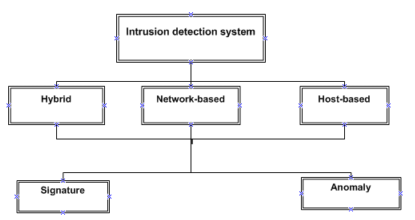
\includegraphics[width=0.5\textwidth]{idsBreakdown.png}
			\caption{A general breakdown of IDS's by Audit System and Event Analysis. Image taken from \cite{Alenezi2012}}
			\label{breakdown}
	\end{figure}
    \subsection{Event Analysis}
   		This section will further subdivide and discuss IDS's by event analysis, which describes the method of detection used, given a particular audit source of data. These detection methods fall into two major categories: \emph{Signature Detection} and \emph{Anomaly Detection}. Signature based methods are much more common in practice, but anomaly detection is an area of much research and promise. A summary of both strategies can be found in figure \ref{comparison}.
   		% Need some citations if we are to claim that signature based methods are more common (like simply typing "E.G." and then giving citations to a bunch of papers describing signature based methods being common).
   		%\ref{comparison} does what, exactly? There's just a 2 there and it is unclear what it is referring to...
	    \subsubsection{Signature Detection} 
	    	Signature Detection is not a simple subject, but much of its difficulty lies in its implementation and not the principles it operates on, meaning that it is easy to understand when thought of in simple terms. Thus, for the sake of easy comprehension, this section is largely a summary of simple descriptions of the principles of Signature Detection from \cite{Taylor2006}, combined with an example for illustration from \cite{Labs1999}. To begin, Signature Detection systems operate on one basic principle: attacks that have been detected before should be recognizable after initially being discovered, assuming that whatever unique feature(s) that identify them are written down and matched against. Thus, a signature-based IDS is one that maintains a database of attack signatures and matches against said database to flag unauthorized or potentially harmful activity on a system, determining if it is an attack at all (and which one it may be of thousands) by examining it side-by-side with each signature. 
	    	
	    	As an example, consider an exploit of Suidperl, a version of Perl that allows the execution of scripts that change user IDs and/or group IDs. Early versions of the Suidperl interpreter do not properly relinquish  root privileges when changing its effective user and group IDs. This allows the creation of a (two line!) script that simply presents the user with a root shell after execution. There are two main approaches to recognize this attack with a signature-based IDS. The first approach is the more simple one, which is searching for strings that have no real use outside of such an attack, and thus can be used to uniquely identify a script that is intended to circumvent access control. The second is to analyze the system and confirm that a valid user-to-root transition has been made, as such sudden access control changes can be clearly identified in file system logs. It is worth noting at this juncture that though both of the above methods are valid to detect the example attack, and both are signature-based, deciding which approach to take is likely based on whether or not the IDS in use is a HIDS or a NIDS. The string-based identification method is better suited for a NIDS, as it can search network activity for strings such as ``\$>=0; \$<=0;" or ``exec (\ae/bin/sh);" that in all likelihood are an exploit attempt and not valid traffic. In contrast, a HIDS could check file systems logs and note that a root shell was spawned without any type of valid user to root transition (a technique called bottleneck verification), and notify authorities accordingly. 
	    	
	    	Naturally, no detection framework is perfect, and Signature Detection, by design, may contain critical flaws depending on how it is implemented. As one might expect, such flaws mostly revolve around the fact that signatures are user-defined and maintained, and firm definitions of what uniquely identifies a signature and what does not is subjective to any given user. Therefore, it is easy to imagine the creation of a signature that defines and identifies a given attack with the utmost precision, but to a fault, such that the signature is so specific that it cannot identify even slight variations of the same attack. Similarly, though probably not as common to see as the previous flaw, signatures can be defined too nebulously. If a signature is not specific enough to a certain attack, and too broadly identifies common attributes between multiple attacks, it is just as problematic as a signature that cannot detect variations of the same attacks. After all, Signature Detection is preferred by some over Anomaly Detection because it triggers less false positives, and a vague signature would completely remove this advantage. 
	    	
	    	Finally, there are two critical and potentially worrisome aspects of signature detection that are extremely important. The first is simple: if the efficacy of the detection system is reliant on the signatures the system has available to match against, then naturally, the system \emph{must be kept up to date.} This means that any and all signature based IDS's require \emph{constant} maintenance to keep them up to date, which is a substantial cost to many organizations seeking to configure an IDS for their network.
	    	
	    	The second is arguably more simple. Mell briefly touches on the fact that Signature Detection methods can only detect known attacks, and thus infers but does not directly discuss an import fact about this type of Event Analysis \cite{Taylor2006}: If signature-based IDS's base the recognition of attacks on whether or not they have seen the attack before \emph{they cannot, by design, ever detect a novel attack}. Thus, signature-based IDS's do not provide complete security, and must be used in addition to an anomaly-based system to detect both new and old attacks.
    	\subsubsection{Anomaly Detection}
    		Anomaly detecting systems work by constructing a system profile of ``normal" behavior, and use that profile to then detect abnormal behavior. The idea is that attacks are a subset of abnormal behavior, which will allow these types of systems to detect them. Most of these systems use some complex statistical analysis to determine when activity differs from the system profile. The major draw to these types of systems is that, unlike signature detection methods, these systems can detect not only variations on known attacks, but completely novel attacks as well. A drawback of this type of functionality is that they are unable to discern intent. They can only flag anomalous behavior, but not the potential cause of that behavior \cite{Mahoney2001}. The other main problem with these systems is that their functionality is predicated on having an effective system profile, which is by no means trivial to produce. They require extensive training sets to learn from, of which few exist. In practice, these types of systems produce large numbers of false positives that require manual inspection to effectively classify as an attack or not. For this reason, few existing systems use this type of detection. Instead, IDS's using this type of detection mechanism are more an an open area of research than production level systems. 
    	\begin{figure}[h!]
			\centering
			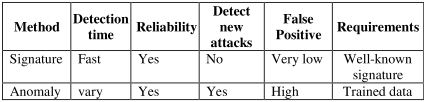
\includegraphics[width=.5\textwidth]{signatreVSanomaly.png}
			\caption{Summary of Event Analysis systems. Image taken from \cite{Alenezi2012}.}
			\label{comparison}
	\end{figure}
\section{Attack Detection by Type}
    % I think we want to model this section after [Bhuyan, Bhattacharyya, Kalitan]
    % Their paper is in the probes section of Mendeley,you should go check it out
    %XXX: NEED MORE IN THIS SECTION
    In this section, we present informal categories of attack we have defined, and how an IDS might identify attacks from this category, in the hopes that some examples might illustrate the inner workings of this complex system with more ease.
    
    \subsection{Probes}
	 This section is will discuss various approaches to detecting Probe attacks. Probes have been classified as any passive information gathering intrusion. The most common form of probe attack, one which will be discussed at length, is the port scan. The motivation for detecting these types of scans is that any intelligent attacker wishing to launch a successful attack will gather background information about the victims system before launching his or her attack. Their primary means of gathering information is by first launching a port scan.
	 
	 There are 65,536 standardly defined ports on a given machine. These are broken down into three large categories: \emph{a.} Well-known ports(0-1,023), \emph{b.} Registered ports (1,024-49,151), \emph{c.} Dynamic and/or private ports (49,152-65,536) [Matiti, P Lecture notes from Surveying Port Scans Methodologies]. %TODO Cite this!
Essentially, a port scan consists of sending a message to each of these ports and analyzing the response message to gain information about what services the victim machine is running. For this reason, TCP ports are the most often scanned because TCP is a connection-oriented protocol, meaning that its response messages are more useful \cite{SilenokElena;RoedelChris;Silenok}. Added to this, it is easy to block/detect UDP traffic at the firewall level \cite{Bhuyan2011}. In general, like most attacks, port scans can be broken down into two high level categories: single source, and distributed source. There is research into detecting both types of scans, with more dedicated to detecting distributed source scans because they are easier to obfuscate and thus harder to detect. Within these high-level categories, \cite{Staniford2002} further divides each of these categories into horizantal, vertical, stobe, and block scans based on the number of machines and ports scanned. A summary of these categories can be found in figure \ref{portScans}.
	\begin{figure}[h!]
		\centering
		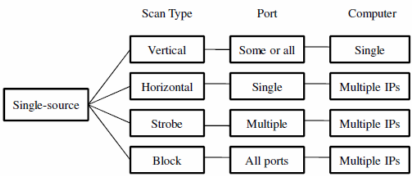
\includegraphics[width=0.45\textwidth]{portScans.png}
		\caption{Summary of Port Scans. Image taken from \cite{Bhuyan2011}}
		\label{portScans}
	\end{figure}
	
	There is a great deal of research into detecting port scans. Several prominent authors' work will be discussed in the following sub section. They have been organized into signature-based, and anomaly-based detection scheme. \cite{Bhuyan2011} presents a much more rigorous and extensive taxonomy of detection methodologies that we leave up to all interested parties to explore. We felt that many of the systems they discuss belong to several of their categories and that a higher level taxonomy made the distinction clearer. 
		\subsubsection{Signature-Based Detection}
		\begin{description}
			\item[Paxon:] %TODO Cite this!
				In this article, the author describes an open-source NIDS called Bro. This system is designed to be a real time, signature based approach to detecting port scans. It relies on the LIBCAP library for capturing network data and is capable of both TCP and UDP processing. It functions by analyzing packet header information to generate what it calls events. These events are \emph{connection attempt, connection established, connection rejected,} and \emph{connection finished}. The preprocessor then passes these events to the analysis engine which alerts the administrator if these events ever cross a certain threshold. It also attempts to detect vertical scans by looking for the one source trying to contact X number of ports in Y amount of time. The main drawbacks to this system are that it drops packets in times of high network traffic load, and produces a high level of false positives. 
			\item[Roesch \cite{Roesch1999}:]
				This article describes the use of another freeware IDS called SNORT. SNORT was designed to be a very lightweight and cost effective solution for companies that needed security, but could not afford a proprietary system. SNORT can function as both a HIDS or NIDS that uses signature based detection. Similarly to Bro, SNORT preprocesses data for before sending it to an analytic engine that matches the data against the signature database. SNORT is one of the most prolific IDS's on the market because of its compatibility, flexibility, and low false positive rate. A drawback to this type of system is scalability. Its primary design was for low stress networks.
						
		\end{description}
		\subsubsection{Anomaly-Based Detection}
		\begin{description}
			\item[Mahoney and Chan \cite{Mahoney2001}:]
				These authors present the NIDS PHAD (Packet Header Anomaly Detection system). It uses a machine learning approach to form normal values for the 33 TCP, IP, UDP, and ICMP packet header fields. The system was trained for 5 days on training data. It then used time differential analysis to assign a probability of attack to incoming packet information. The system was tested for 10 days on the 1999 offline DARPA packet test data set and was able to detect 67 of 201 listed attacks with a false positive rate of 10 per day.
			\item[Ertoz \emph{et al.} \cite{Ertoz2003}:]
				The authors present a system called MINDS (Minnesota Intrusion Detection System). It uses NetFlow for network traffic monitoring so that it can analyze flow level information, packet source/destination characteristics, and packet size. It uses a data mining approach to compare trends in network data flow with its system profile. The events that it analyzes are assigned an anomaly score, which are the systems' criteria for alerting the system administrator. It was shown to have comparable performance to SNORT and was said to be able to detect stealthy port scans, but little to no data was supplied on its effectiveness in this area.
			\item[Streilein \emph{et al.} \cite{Attacks2002}:]
			The authors describe a system for detecting stealthy port scans and Denial of Service attacks. Their system is a tabling approach that keeps track of connection statistics such as time, source,and  destination. A series of artificial neural networks are used to analyze the data for anomalous behavior. Their system was trained on the 1998 and 1999 DARPA training data sets and was shown to have a detection rate of 100\% and relative false positive rate of 0.1\%. These results show promise, but not as much as it might seem due to the strong criticisms of their chosen data set. We present theses criticisms in the discussion section. 			
		\end{description}
		
		\subsubsection{Analysis}

    \subsection{Privilege Escalation} %Worth noting here that category "Privilege Escalation" is semi-arbitrary, IE not a formal category (that, or just cover it in discussion section).
    	Privilege Escalation attacks are described in two general categories in this paper: Remote to User Attacks and User to Root Attacks. In the broadest sense, Remote to User Attacks are when an attacker seeks to gain local user access to a machine that they have network access to. A User to Root Attack, as one may infer from its name, is when an attacker who already possesses local user access seeks to escalate their privileges to those of a root user, IE gain root user access. In the following sections, both types of attacks are explained in detail. Note that these categories are not formal or standard categories defined in the field, but ones created by us for the sake of clarity. For more information on why a standard taxonomy was not used, see section \ref{categorization}.
    \subsubsection{Remote to User}
    	A Remote to User attack, as explained by \cite{Labs1999}, is when an attacker who has network access to a system but does not have an account on that machine exploits a vulnerability on the system to gain unauthorized local access as a user of the target system. These types of attacks come in many forms, and can be as simple as getting valid user authentication information through guessing a user's password with a dictionary attack. However, just as common are attacks that exploit a vulnerability in a common and innocuous system service, such as FTP to gain local user access. These exploits can change system settings to allow an attacker remote access, but they can also trigger buffer overflows, which in many circumstances allow an attacker to execute arbitrary code on the remote host (which is often used to gain root access, as we will discuss later). 
    \subsubsection{User to Root}
     	A User to Root attack, also summarized from \cite{Labs1999}, is when an attacker who has no access or local user access to a system escalates their privileges to those of a root user. As with Remote to User attacks, User to Root attacks can come in a wide variety of formats. However, most of them tend to be some form of vulnerability exploit that either allows temporary root access (which is enough for any attacker to establish a backdoor for themselves for root access in the future), or triggers a buffer overflow, which can be used by a clever attacker to execute arbitrary code to gain root access. Buffer overflows are an extremely common way vulnerability to exploit, both to gain root access but to just gain local user access as well.
     \subsubsection{Detection}
     	Currently, research on detection of Privilege Escalation attacks is fairly rudimentary. Such attacks are often readily recognizable to signature-based IDS's, regardless of whether they lie on the network or the host. As was briefly mentioned in our explanation of signature-based IDS's, \cite{Labs1999} shows, through copious examples of attacks, what a signature for each would have to include (though it is worth noting, such attacks are from the late 90's, and are thus quite out of date as examples). However, the details of how an anomaly based IDS would detect such attacks is not touched upon. With the massive variety of approaches attackers have found to escalate their privileges, one could surmise that anomaly based methods of detection would prove ineffective. Moreover, general research on detection of Privilege Escalation attacks is essentially non-existent, or obscure enough to locate that we have not found papers on it. To summarize, much research at this juncture is focused on intrusion \emph{prevention} instead of detection, which revolves around building a more robust and secure network and system. In the course of my research, I could not find any papers categorizing Privilege Escalation attacks into types, nor any papers discussing how to formally recognize them and detect them. For more detailed analysis of the issues with research on this specific aspect of intrusion detection, see section \ref{categorization}.
     
    \subsection{Denial of Service}
    	This section will discuss the current detection methodologies for Denial of Service (DoS) attacks. It will begin with a discussion about prominent types of attacks and how they are carried out. Then, it will move into a summary of various researchers' work on detecting these very difficult to detect attacks. %TODO make sure that you keep this paragraph true to how you actually write this section
    	
    	We classify DoS attacks as any attack whose goal is to tie up a resource on the victims machine. The types of attacks can be broadly classified as \emph{software exploits} and \emph{flood attacks.} This section will focus on flood attacks because the majority of software exploit attacks can be solved by keeping one's system up to date with all software patches \cite{Hussain2003}. 
    	
    	One of the open problems in studying this type of attack is that there is no standard taxonomy describing the breakdown of the various types. Here, we present Specht and Lee's taxonomy for classifying attacks because we felt that it was the most complete and easy to understand. The following descriptions where originally described by them in \cite{Specht2004} a summary of which can be found in figure \ref{breakdown2}. DoS attacks can, at a high level, be classified as single source or multi-source, where the latter are referred to as Distributed Denial of Service (DDoS) attacks. DDoS attacks are becoming more and more common as they are a powerful means of launching an attack and are harder to trace. The following categories apply to both single-source DoS and DDos attacks.
    		\subsubsection{Flood Attacks}
    		Flood attacks are characterized by compromised systems (zombies) sending large amounts of network traffic to a victim machine. This overload of traffic causes the victim's system to slow down to an unusable level or crash entirely. The most commonly used protocols for this type of attack are UDP and ICMP. In a UDP flood attack, large amounts of UDP packets are sent to either random or sometimes specific ports on the victims machine. The victim machine tries to determine which application is requesting connections and thus ties up all its resources. 
    		
    		During and ICMP attack, zombies send large amounts of ICMP ECHO REPLY packets to the victim machine. The victim's system then tries to reply to all of the incoming traffic, but can not handle the load and crashes. It is worth noting that both of these types of attacks can be avoided with proper network configuration. For example, blocking UDP traffic or not reply to ping messages in the default manner.
    		\subsubsection{Amplification Attacks}
    		An amplification attack is carried out by sending a message to the broadcast address withing a network, and spoofing the return address to that of the victims machine. Other author's have termed this type of attack a \emph{reflector attack} \cite{Hussain2003}. Two common examples of this type of attack are the \emph{smurf} and \emph{Fraggle} attack. 
    		
    		During a smurf attack, ICMP ECHO REPLY packets are sent to a network amplifier with a spoofed return address. During a fraggle attack, UDP ECHO packets are sent to a network amplifier and the victim's echo port and character generation port are spoofed as return the address. This causes the the victim's system to enter and infinite loop where the character generation port sends packets to the echo port and so on and so forth.
    		\subsubsection{Protocol Exploit Attacks}
    		These types of attacks take advantage of an inherit flaw in a particular network protocol's design. In this way, examples are the best way to understand these types of attacks, so we present two: TCP SYN, and PUSH ACK attacks. 
    		
    		During a TCP SYN attack, the attacker or attackers will send illegitimate TCP Synchronization message with a spoofed IP return address to the victims machine. The victim will then  reply to the message, the second step in the handshake process, but because the return address is spoofed, no reply will ever come back. The victim machine will then be stuck trying to maintain this growing number of open, but incomplete, connections. Eventually, the victim's machine will run out of buffer space and will thus be unable to respond to legitimate traffic.
    		
    		In a PUSH ACK attack, the attacker or attackers send TCP packets with both the PUSH and ACK fields set to one. This causes the victim machine to dump all buffered TCP data and send an acknowledgment when done. If enough of these calls are made within the victim system, it will eventually run out of processing power and crash.
    		\subsubsection{Malformed Packet Attacks}
    		These types of attacks are characterized by an attacker sending malformed packets to the victims system in order to lock up its computing resources. For example, a packet can be set to have the same source and destination IP addresses to confuse the victims system, or all quality control bits can be set to one so that the victim's system must use extra resources to process the packets. The goal being that if enough of these packets are sent, the victims system will crash or become unable to handle legitimate traffic.
    		\begin{figure}[h!]
				\centering
				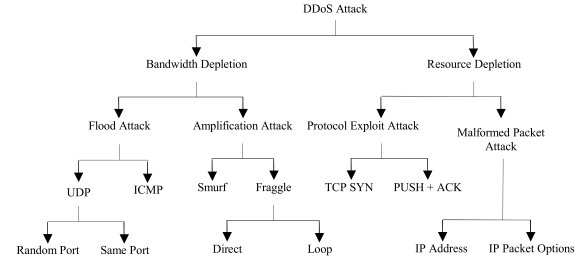
\includegraphics[width=0.5\textwidth]{doSBreakdown.png}
				\caption{A summary of the different types of DoS attacks \cite{Specht2004}}
				\label{breakdown2}
 			\end{figure}
		\subsubsection{Detection Methodologies} 
		DoS attacks are notoriously hard to detect and prevent. This difficulty is due to the fact that they take advantage of existing architectural implementation. We present three approaches to trying to solve this problem or related sub-problem, but it is worth noting that currently there is no comprehensive solution to detecting or defending against all known forms of DoS attacks \cite{Specht2004}. No strictly signature-based detection methods will be discussed because multiple authors, \cite{T.2009}, \cite{R.2004}, \cite{G.2006}, argue that signature-based methods are ineffective for detecting these types of attacks. However, one author, \cite{Alenezi2012}, did make the case that simple DoS attacks can be detected using signature-based methods. While there is merit to this argument, these are not the types of attacks that most systems are worried about. Any attack of considerable risk must be detected using anomaly-based detection.
		\begin{description}
			\item{Labib and Vemuri \cite{Labib2004}:} They use multivariate statistical approaches to detect DDoS and Neptune probe attacks with a focus on real time detection. More specifically, they use Principle Component Analysis to reduce the multidementional space represented by network feature vectors for real time analysis. They are able to detect 100\% of attacks in the DARPA 1998 data set, however, as noted earlier, the data set that they tested on has been criticized of being unsatisfactory. \emph{See Section \ref{trainingSets}}. A more exhaustive discussion on DoS attack detection can be found in \cite{Alenezi2012}.
			\item{You, Zulkrnine, and Haque \cite{}:} %Need citation  
			These authors present a system that detects DoS attacks by analyzing differences in distances. The Time to Live (TTL) field is used to infer the distance away that a packet originated because it is usually a field that is automatically filled by the kernel and not often spoofed by attackers. A normal system distance profile is built using the average TTL value over a period of time. This information is compared with traffic arrival rates, and the correlation between the two is used to detect anomalous behavior. Both normal and abnormal looking traffic are determined by use of the mean absolute deviation. The difficulties that this approach encountered was that a clever attacker would be able to spoof the TTL packets in such a way that they would not be detected, and that network traffic routes are constantly changing, so TTL is not always an accurate representation of the distance that a packet has traveled.
			\item{Hussain, Heidemann, and Papadopoulos \cite{Hussain2003}:} These authors present two methods for not only detecting DDoS attacks, but also for trying to distinguish between single source DoS attacks and DDoS attacks. They attempt to distinguish between the two by looking for what they term \emph{ramp up behavior}. Their theory is that a spike in network behavior would happen when an attack command is issues to the zombies in a DDoS attack. This ramp up in activity would be much more noticeable in DDoS attacks than in a single source DoS attack. Admittedly, this is not a very robust method of detecting attack, but it shows some promise. The also describe using spectral analysis on packet arrival rates to distinguish between the two types of attacks. They find that single source DoS attacks show a characteristic high frequency linear trend, while DDoS attacks are dominated by low frequency trends. They are then able to distinguish between the two using data visualization techniques. They deploy their systems on the Los Nettos ISP in Los Angeles and USC's secondary internet connection. They are able to detect 98 attacks between the two sites. Unfortunately, their system has not been tested in a controlled environment and as such has not yet been integrated into a full IDS system.
		\end{description}
  
\section{Discussion}
    % What would we say here?
    In the following section, we discuss open problems in the field, difficulties faced in our research that effected our results, and current knowledge gaps in Intrusion Detection that we believe need to be addressed.
    
    \subsection{Open Problems}
    After conducting our research we have found several shortcomings within this research field. This section will describe what we see as open research problems that have the potential to make significant contributions to this field.
    	\subsubsection{Training Sets} \label{trainingSets}
    	In the course of our research, there were several points where we discovered current work in the field is underdeveloped, heavily criticized, or lacking in some way. Training sets of network traffic for IDS's were of the largest sections of our research where we discovered this, as we learned that there is essentially only one training set that is moderately successful in gauging the efficacy of an IDS (the 1999 DARPA training set), and it is heavily criticized nonetheless. 
    	
    	Brugger \emph{et al} \cite{Brugger2007} perform a survey of authors critiquing the DARPA evaluation, who describe the flaws in the training set from a variety of angles. One of the biggest criticisms of the training set (McHugh via \cite{Brugger2007}) is that it did not accurately model/simulate a real-world network. This is quite poignant, as a realistic simulation of a real-world network is absolutely crucial if one's intent is to gauge how effective a given IDS would be at detecting attacks in a real-world scenario. Naturally, this is difficult to do effectively, as it begs the question: what makes a given simulation of network traffic ``realistic"? Human users are unpredictable, and in all likelihood, any network with actual users on it may look widely different from one day to the next. How does one account for these differences when artificially creating network traffic full of attacks to gauge the efficacy of an IDS on? 
    	
    	Realistic simulation of network traffic is a large enough critique on its own to render the DARPA dataset inadmissible as a standard gauge for IDS efficacy, but that is only one of many ``flaws" contained in the set, according to \cite{Brugger2007}. Brugger \emph{et al} \cite{Brugger2007} surveyed authors and found critiques like the one seen above, but they \emph{also} tested the dataset themselves against Snort, one of the most widely recognized ``off-the-shelf" IDS's. Their reason for choosing Snort in particular was both because of how recognized it was, but also because they believed the dataset would prove to be ill-equipped for gauging the efficacy of a signature-based system, which Snort is also known for. They were correct in this assumption, as, over the course of their research, they discovered that ``...the dataset only includes a very limited number of attacks that are detectable with a fixed signature" \cite{Brugger2007}. 
    	
    	Thus the DARPA dataset has been demonstrated as both ineffective at simulating network traffic and at testing signature-based IDS's like Snort, which are some of the most commonly used IDS's today \cite{Taylor2006}. We feel that if a proper data set was ever produced, it would greatly aid in the comparability and effectiveness of testing IDS systems.
    	\subsubsection{Categorizing Attacks} \label{categorization}
    	As briefly mentioned in our section on Privilege Escalation, the formal categorization of cyber attacks, how they work, and therefore how to defend against them, is a field in and of itself (referred to from here on as Attack Taxonomy). What this means is that summarizing a complex field such as Intrusion Detection is already difficult, and an additional layer of difficulty is added when one realizes that a formally defined and agreed upon taxonomy of attacks does not exist. Without such a taxonomy, examples and descriptions of how certain IDS's detect certain types of attacks, naturally, becomes harder to describe. This can be amplified by the fact that certain categories have significantly more research available on them. Probes, for example, having an existing general taxonomy that we could locate \cite{Bhuyan2011}, as opposed to Privilege Escalation, which is largely a field of research on prevention instead of detection, and thus did not have an easy to find taxonomy. 
    	
    	Of course, taxonomies that \emph{could} have been selected for the purpose of our paper and used for the sake of explanation do exist. It is not as if we could \emph{only} appropriate a taxonomy if Attack Taxonomy experts had one that they collectively preferred to use as a ``community standard". However, given our time constraints and the sheer complexity of available taxonomies, we were not able to spend the time doing the additional research to determine which taxonomy might apply best to our survey of Intrusion Detection. Hansman et al. \cite{Hansman2005} provided an insightful look into existing taxonomies and their advantages/disadvantages, but also illustrated that the depth of Attack Taxonomy research as a whole means we cannot simply ``choose a taxonomy". 
    	
    	As our research progressed, we realized that a taxonomy was not ultimately necessary for an easy explanation of Privilege Escalation type attacks, but that we did need to explain them somehow. What was interesting was that, in the course of this research, we expected to find enough contextual information about the field that we could adequately describe how detection of these attacks worked. We found such context, but in addition, we discovered precisely how lacking research on \emph{detection} of Privilege Escalation attacks is, and how research around them instead focuses on \emph{prevention}. That is not to say that research on detection of Privilege Escalation attacks does not exist, but it did tend to focus on individual Privilege Escalation attacks at a time (e.g.\cite{Hsu2006} or \cite{Kuperman2005} on buffer overflow attacks) instead of the category as a whole. Moreover, research we could find that focused on the entire category of Privilege Escalation attacks was where this focus on prevention was most prevalent. Referring to what we call Privilege Escalation attacks as ``Access Control Vulnerabilities", Sun et al. \cite{Sun2011} provide a good example of this, as they focus on \emph{detecting vulnerabilities in a specific system}, with the idea being that they can then be patched up to prevent harmful attacks (\cite{Livshits2005} and \cite{Dalton2009} both follow this same format). Ultimately, we found a large hole in the body of research around Privilege Escalation attacks/Access Control vulnerabilities, where the detection of said attacks seems like it requires significant research if IDS's are going to become even moderately successful at finding Privilege Escalation attacks as they occur.
    	\subsubsection{DoS Detection}
    	As noted previously, there is no comprehensive solution for DoS detection \cite{Specht2004}. There are a vast number of experimental methods out there, of which we have presented three in this paper. However the most pervasive form of detection is having a skilled network administrator and a host of preventative measures. We feel that several anomaly detection-based methods, namely ramp up behavior and spectral frequency analysis \cite{Hussain2003}, have shown promise in detection of these types of attacks and that more research into this area is vital to be able to automate detection and thus defenses against DoS attacks.
    \subsection{IDS's In Practice}
    	There are some important conclusions about IDS's to take away that do not belong in their definition section that we have decided to include here. 
    	\subsubsection{Limitations of IDS's}
			This section describes general limitations and draw backs of all IDS systems, regardless of audit system or event analysis. These should be taken into account by anyone attempting to employ the use of an IDS.
    		\begin{enumerate}
    			\item Scalability. There is a large human component that is required to keep an IDS in operation, and the larger a system is, the more sensors it needs, the more data is generated that needs to be evaluated, the more staff is required and man hours needed for effective analysis.
    			\item False Positives. Improperly configured IDS's generate a high number of false positives that require an IT analyst to be sorted out.
    			\item Vulnerable. Most IDS's are not insulated from attacks themselves, and can be disabled by clever attackers.
    			\item Maintenance. No IDS comes ready to use, and must be configured to meet the specifications of its assigned environment. In addition, IDS's must be maintained by skilled personnel to achieve maximum efficacy.
    			\item Always Behind. New attacks are generated quicker than IDS's can detect them.
    		\end{enumerate}
    	\subsubsection{Effective Defense}
    		It is worth of note that, effectively employed, IDS's can be used to automate defense, but any organization looking to install a comprehensive security system needs to analyze their potential risk and determine what is necessary to install, as there is no comprehensive IDS. A combination of host-based and network-based systems must be used for complete detection coverage, but IDS's only \emph{detect} attacks, they do nothing to prevent them, and a prevention system \emph{and} talented and reactive IT staff are required for an IDS's usefulness to be fully realized. 
\section{Limitations and Extensions}
	One large limitation in the Privilege Escalation section was proper research of bottleneck verification. Bottleneck verification, as we understand from contextual uses of it in reports on cyber attacks, is an attempt at intrusion detection through confirming on the host, with the use of system logs, that a user made a valid transition from user access to root access. In a perfect world, looking at the system logs should tell us if a user authenticated properly to gain root access, and if there is a gap between user and root access that is not filled with some variation of valid privilege escalation (such as authentication), then an IDS can raise a flag. Sadly, our time and scope limitations prevented us from delving into research into this concept in greater detail, as it may have answered some of our questions about successful detection of Privilege Escalation/Access Control attacks (see discussion section for said questions). It is worth noting that a brief sojourn was made to try and find the basics of the concept, but it became immediately clear to us that it would not be a simple concept that could be examined with ease and included in our final results. This concept was one of many casualties that we wished to include, but could not find easily summarized in any paper. Therefore, it would have been an interesting concept to explore, as it was essentially an example from a different subset of research of the complex principles we would like to see briefly and succinctly explained, hopefully not unlike our explanation of IDS's.
\section{Conclusion}
    % See outline for this bit
    % Outline seems to just describe discussion section(s). How do we want to conclude? What did we learn?
    Through our research into Intrusion Detection, we have gained a basic understanding of the field and its limitations. Although that understanding is shallow, we hope that gathering the building blocks of Intrusion Detection into one place might help others who wish to learn more about the field be able to pick up the basics with greater ease. In addition, we believe that the flaws and research gaps we have discovered, or thought to have discovered, might illustrate to professionals in the field what their research looks like to those with an introductory understanding of Intrusion Detection. 

	% References-------------------------------
	%I produced all references, we invariably wont use all of them, but this makes it easier to cite things trhoughout the paper. At the end, we will re-Export the bibTex, to just be what we used by searching through this document for the work 'cite'
	
% The following two commands are all you need in the
% initial runs of your .tex file to
% produce the bibliography for the citations in your paper.
\bibliographystyle{abbrv}
\bibliography{allSources}{}  % sigproc.bib is the name of the Bibliography in this case
\nocite{*}
% You must have a proper ".bib" file
%  and remember to run:
% latex bibtex latex latex
% to resolve all references
%
% ACM needs 'a single self-contained file'!
%
\balancecolumns
\end{document}
